%%%  Template to prepare a defense of Bc./Mgr./... thesis
%%%  to be presented at MFF
%%%  (unofficial)
%%%
%%%  AUTHOR:  Arnošt Komárek
%%%           Department of Probability and Mathematical Statistics
%%%           Faculty of Mathematics and Physics, Charles University in Prague
%%%
%%%  LOG:    20150505  created by modification of some previous personal presentations
%%%          20170522  update related to new MFF logo
%%%  
%%%  ===========================================================================
\documentclass[c, 10pt]{beamer}


%%%%% Package needed if some accented letters in the presentation
%%%%% -------------------------------------------------------------
\usepackage[utf8]{inputenc}


%%%%% Most beamer settings and other LaTeX commands
%%%%% are provided in the file below
%%%%% -----------------------------------------------------
%%%
%%%  Style for MFF related presentations
%%%  (unofficial)
%%%
%%%  AUTHOR:  Arnošt Komárek
%%%           Department of Probability and Mathematical Statistics
%%%           Faculty of Mathematics and Physics, Charles University in Prague
%%%
%%%  LOG:    20150430  created by modification of some previous personal presentations
%%%          20170522  modified (new MFF logo)
%%%  
%%%  ===========================================================================

%%%%% If to determine whether Czech or English version
%%%%% of a presentation is to be produced
%%%%% default = Czech
%%%%% ------------------------------------------------------
\newif\ifCZversion
\CZversiontrue

\ifCZversion\else\renewcommand{\uv}[1]{``#1''}\fi


%%%%% Included packages
%%%%% ----------------------------------------------------------
\usepackage{helvet}                       % font
\usepackage{amsmath, amssymb}
\usepackage{delarray}
\usepackage{multicol}
\usepackage{graphicx, fancybox}
\usepackage{psfrag}
\usepackage{fancyvrb}
\usepackage{eurosym}
\usepackage{bbding}
%\usepackage{marvosym}
\usepackage{wasysym}
\usepackage[czech]{babel}
\usepackage{mathrsfs}
\usepackage[pdftex]{bookmark}

\usepackage{bbm}	% For lowercase blackboard bold
\usepackage{multicol}  	% ultiple columns
\usepackage{enumerate}

%%%%% Some LaTeX commands
%%%%% ----------------------------------------------------------
\renewcommand{\arraystretch}{1.2}


%%%%% Some colors and related commands
%%%%% ----------------------------------------------------------

  %% Pantone 186 = "official" red of MFF
\definecolor{redmff}{rgb}{0.7892720,0.0651341,0.1455939}          

  %% First level color = black
\definecolor{colOne}{rgb}{0,0,0}
\newcommand{\tOne}[1]{\textcolor{colOne}{#1}}
\newcommand{\tOneb}[1]{\textcolor{colOne}{\textbf{#1}}}
\newcommand{\tOnei}[1]{\textcolor{colOne}{\textit{#1}}}

  %% Second level color = quite dark blue
\definecolor{colTwo}{rgb}{0,0,0.3}                
\newcommand{\tTwo}[1]{\textcolor{colTwo}{#1}}
\newcommand{\tTwob}[1]{\textcolor{colTwo}{\textbf{#1}}}
\newcommand{\tTwoi}[1]{\textcolor{colTwo}{\textit{#1}}}

  %% Third level color = something between blue3 and blue4
\definecolor{colThree}{rgb}{0,0,0.7}              
\newcommand{\tThree}[1]{\textcolor{colThree}{#1}}
\newcommand{\tThreeb}[1]{\textcolor{colThree}{\textbf{#1}}}
\newcommand{\tThreei}[1]{\textcolor{colThree}{\textit{#1}}}

  %% Color to alert (highlight) = MFF red
\definecolor{alertCol}{rgb}{0.7892720,0.0651341,0.1455939}
\newcommand{\tal}[1]{\alert{#1}}
\newcommand{\talb}[1]{\textbf{\alert{#1}}}
\newcommand{\tali}[1]{\textit{\alert{#1}}}

  %% White
\newcommand{\tw}[1]{\textcolor{white}{#1}}
\newcommand{\twb}[1]{\textcolor{white}{\textbf{#1}}}
\newcommand{\twi}[1]{\textcolor{white}{\textit{#1}}}

  %% Some other colors used somewhere
\definecolor{semiwhite}{gray}{0.98}
\definecolor{mffgray}{gray}{0.95}
\definecolor{semiblack}{gray}{0.5}
\definecolor{rred}{rgb}{0.5,0,0}


%%%%% Beamer stuff
%%%%% ----------------------------------------------------------
\mode<presentation> {

    %%% General theme of a presentation (some pre-specified themes)
    %%% ------------------------------------------------------------------
    %\usetheme{CambridgeUS}
    \usetheme{Warsaw}

    %%% Color schemes that will be used unless redefined below
    %%% ------------------------------------------------------------------
    %\usecolortheme{wolverine}
    \usecolortheme{beaver}


    %%% Color schemes for different elements of a presentation
    %%% ---------------------------------------------------------

      %%% Uncomment the two rows below if some background file (layout) is to be used
      %%% on all slides
    %\usebackgroundtemplate{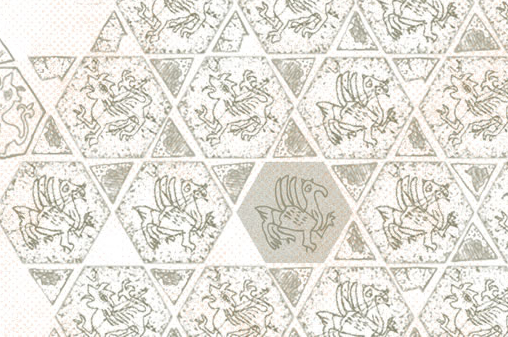
\includegraphics[width=\paperwidth, height=\paperheight]{./FigureLayout/BackgroundRotunda}}
    %\setbeamercolor{background canvas}{bg=}                                                             

      %%% Setting for "standard" slides
      %%% - must be commented if background file used
    \setbeamertemplate{background canvas}[vertical shading][bottom=semiwhite, top=white, middle=semiwhite!50!white]
    \setbeamercolor{background canvas}{bg=white}                           %% NO EFFECT WHEN \setbeamertemplate{background canvas} WAS USED

      %%% Colors of frametitle, normal, alerted and math texts
    \setbeamercolor{frametitle}{fg=white, bg=redmff}
    \setbeamercolor{normal text}{fg=black}
    \setbeamercolor{alerted text}{fg=redmff}
    \setbeamercolor{math text inlined}{fg=colTwo}
    \setbeamercolor{math text displayed}{fg=colTwo}

      %%% Colors for some special boxes defined below
    \setbeamercolor{mffboxcol}{fg=colTwo, bg=mffgray}
    \setbeamercolor{mffboxcolupper}{fg=white, bg=redmff}

    %%% Set serif font (patkové písmo) in mathematics
    %%% ------------------------------------------------
    %\usefonttheme[onlymath]{serif}

    %%% Itemize style (rectangles instead of bullets)
    %%% ------------------------------------------------
    % \useinnertheme{rectangles}

    %%% Default content of a header of each slide
    %%% (currently nothing)
    %%% ------------------------------------------------
    \setbeamertemplate{headline}{}

    %%% Default content of a foot of each slide
    %%% ------------------------------------------------
    %\setbeamercolor{page number in head/foot}{fg=black, bg=white}
    \setbeamertemplate{footline}{
      \hspace*{2.5em}
      \begin{beamercolorbox}{section in head/foot}
      \vskip1pt
      \tOne{\rule{\textwidth}{1pt}}
      \vskip2pt

      %%% Foot containing (a) page number/total number of pages, (b) name, (c) short title of presentation
      {\small \tOne{\insertframenumber}\textcolor{semiblack}{/\inserttotalframenumber}}\hspace{1em}
      \tOne{\footnotesize \insertauthor}\hfill
      \textcolor{redmff}{\footnotesize\insertshorttitle\hspace{3em}}

      %%% Foot containing (a) page number/total number of pages, (b) name, (c) short section title
      %{\small \tOne{\insertframenumber}\textcolor{semiblack}{/\inserttotalframenumber}}\hspace{1em}
      %\tOne{\footnotesize \insertauthor}\hfill
      %\textcolor{redmff}{\footnotesize\thesection. \insertsection\hspace{3em}}
    
      \hspace*{3.5em}
      \vskip3pt
      \end{beamercolorbox}
    }

    %%% Title page
    %%% -------------------
    \setbeamertemplate{title page}{
      %\vspace*{-0.5em}
      \begin{center}
      \textcolor{black}{\normalsize\bfseries\rmfamily \insertinstitute}

      \vspace{1em}
        
      \ifCZversion
        
\includegraphics[width=0.8\textwidth]{./FigureLayout/mff_cz_color}
      \else
        
\includegraphics[width=0.8\textwidth]{./FigureLayout/mff_en_color}
      \fi

      \medskip
      \noindent\textcolor{redmff}{\rule{\textwidth}{2pt}}
  
      \bigskip
      \textcolor{black}{\normalsize\bfseries \insertauthor} \\[0.5ex]

      \bigskip
      \textcolor{redmff}{\Large\bfseries \inserttitle}

      \medskip
      \textcolor{redmff}{\large\insertsubtitle}

      \medskip
      \noindent\textcolor{redmff}{\rule{\textwidth}{2pt}}
      
      \medskip
      \textcolor{colTwo}{\small \insertdate}
      \end{center}
    }    

    %%% Switch-off/on foot with navigation symbols    
    %%% -----------------------------------------------
    % \setbeamertemplate{navigation symbols}{}
    \usenavigationsymbolstemplate{}

    %%% Left and right margin
    %%% --------------------------------
    %\setbeamersize{text margin left=1cm}
    %\setbeamersize{text margin right=1cm}


    %%% Use of a logo on each slide
    %%% (not really recommended, so commented)
    %\logo{
\includegraphics[height=1.5cm, width=1.5cm]{./FigureLayout/mff_logo}}
}


%%%%% Commands to produce slides at the beginning of each section
%%%%% --------------------------------------------------------------
\renewcommand{\thesection}{\arabic{section}}
\newcommand{\framesection}{
  \begin{frame}%[plain]

  \vspace*{2em}
  \begin{center}\Large
  \ifCZversion Oddíl \thesection \else Section \thesection \fi
  \end{center}

  \begin{center}\color{rred}\Large
  \insertsection
  \end{center}

  \end{frame}
}


%%%%% Style for software related stuff
%%%%% ----------------------------------------------------------
\newcommand{\Rko}{
\includegraphics[width=5.094mm, height=3.876mm]{./FigureLayout/Rlogo}}
\newcommand{\Rfun}[1]{\textcolor{redmff}{\texttt{#1}}}

\DefineVerbatimEnvironment{Rin}{Verbatim}{formatcom=\color{redmff}, fontsize=\scriptsize, frame=single, framerule=1pt, framesep=2pt}
\DefineVerbatimEnvironment{Rout}{Verbatim}{formatcom=\color{blue}, fontsize=\scriptsize, frame=single, framerule=1pt, framesep=2pt}


%%%%% Boxes
%%%%% ----------------------------------------------------------
\newcommand{\mffbox}[2][0pt]{%
  \begin{beamercolorbox}[center, sep=#1, rounded=true, shadow=true]{mffboxcol}
  #2
  \end{beamercolorbox}
}

\newcommand{\mffboxTitle}[2]{%
  \begin{beamerboxesrounded}[lower=mffboxcol, upper=mffboxcolupper, shadow=true]{#1}
  #2
  \end{beamerboxesrounded}
}


%%%%% Some constructions for displayed math
%%%%% ----------------------------------------------------------
\newcommand{\dmath}[2][-1.4em]{%
  \begin{beamercolorbox}[center, sep=#1, rounded=true, shadow=true]{mffboxcol}
  \begin{displaymath}
  #2
  \end{displaymath}
  \end{beamercolorbox}
}

\newcommand{\dalign}[2][-1.4em]{%
  \begin{beamercolorbox}[center, sep=#1, rounded=true, shadow=true]{mffboxcol}
  \begin{align*}
  #2
  \end{align*}
  \end{beamercolorbox}
}

\newcommand{\dgather}[2][-1.4em]{%
  \begin{beamercolorbox}[center, sep=#1, rounded=true, shadow=true]{mffboxcol}
  \begin{gather*}
  #2
  \end{gather*}
  \end{beamercolorbox}
}



%%%%% \ifCZversion is defined inside MFF_Present.sty
%%%%% to distinguish between Czech and English presentations
%%%%% ------------------------------------------------------
%\CZversiontrue       %% for presentations in Czech (Slovak)
\CZversionfalse      %% for presentations in English


%%%%% Uncomment appropriate choice below if you wish to create
%%%%% notes for audience having 2 or 4 slides on each (A4) page.
%%%%% -------------------------------------------------------------
\usepackage{pgfpages}
%\pgfpagesuselayout{4 on 1}[a4paper, landscape, border shrink=5mm]
%\pgfpagesuselayout{2 on 1}[a4paper, border shrink=5mm]


%%%%% Basic settings of the document
%%%%% (will be automatically used to create a title page, foots etc.)
%%%%% --------------------------------------------------------------------

  %%% Main title
  %%% - short and long version
  %%%   --> will appear on place where \inserttitle and \insertshorttitle commands used
  %%%   --> if the full title is short enough, both short and long versions might be the same
\title[Gibbs-Delaunay Tessellations]{%                       
       Gibbs-Delaunay Tessellations}

  %%% Subtitle (comment it if you do not want to have it)
  %%%   --> will appear on place where \insertsubtitle and \insertshortsubtitle commands used
 \subtitle[]{Simulation and estimation}

  %%% Author
  %%% - as "short" version, link to the author's webpage is used
  %%%   (e.g., e-mail is also a useful alternative)
  %%%   --> will appear on places where \insertauthor and \insertshortauthor commands used
\author[jahn@karlin.mff.cuni.cz]{%
        Daniel Jahn}

  %%% Author's affiliation
  %%% - can be fully commented for defense presentation
  %%%   --> will appear on places where \insertinstitute and \insertshortinstitute commands used
\institute[KPMS]{%
           Department of Probability and Mathematical Statistics}

  %%% Date of presentation
  %%% - replace it by real date in case of a defense presentation
  %%%   --> will appear on places where \insertdate and \insertshortdate commands used
\date[12.9.2018]{%
      12. September 2018}


\begin{document}

%%%%% Title slide
%%%%% =====================================================================================
\frame[plain]{\titlepage}


%%%%% Slide
% ----------------------------------------------------------------------------------------
\section{Point processes}
\framesection{}

%%%%% Slide
% ----------------------------------------------------------------------------------------
\begin{frame}\frametitle{Poisson point process}
We're on $(\mathbb R^d, \mathcal B)$, Euclidean space, $\lambda^d$ Lebesgue measure.\newline
Denote $\mathcal B_0$ the set of bounded Borel sets. \newline

\mffboxTitle{\textbf{Definition}. Poisson point process}{
Let $\mu$ be a locally finite non-atomic measure on $\mathbb R^d$. A point process $\Phi$ satisfying 
\begin{itemize}
    \item $\Phi(B) \sim Pois(\mu(B))$ for each $B \in \mathcal B_0$,
    \item $\Phi(B_1), \dots, \Phi(B_n)$ are independent for each $n \in \mathbb N$ and $B_1,\dots, B_n \in \mathcal B_0$ pairwise disjoint.
\end{itemize}
is called a \alert{Poisson point process} with the \alert{intensity measure} $\mu$.
}
\vspace{3mm}
If $\mu = z \lambda^d$ we call the process \alert{homogenous} and $z$ the \alert{intensity}.

For $\Lambda \in \mathcal B_0$, denote the distribution of $\Phi \cap \Lambda$ as $\pi_\Lambda^z$. 

For the case $z=1$, use $\pi_\Lambda$.

\end{frame}



%%%%% Slide
% ----------------------------------------------------------------------------------------
\begin{frame}\frametitle{Poisson point process as a reference measure}
$\Phi: (\Omega, \mathcal A, P) \to (\mathcal F_{lf}, \mathscr F)$ where 
\begin{itemize}
\item $\mathcal F_{lf} = \{ \gamma \subset \mathbb R^d | \; \gamma \cap \Lambda \text{ is finite for all } \Lambda \in \mathcal B_0\}$ and 
\item $\mathscr F$ is generated by sets of the form $\{\gamma \in \mathcal F_{lf} | \; N_\Lambda(\gamma) = n \}, n \in \mathbb N, \Lambda \in \mathcal B$, where $N_\Lambda(\gamma) = \text{Card}(\gamma \cap \Lambda)$.
\end{itemize}
\vspace{3mm}

We can view $\pi_\Lambda$ as a reference measure on $(\mathcal F_{lf}, \mathscr F, \pi_\Lambda)$.

Then we can define new point processes through defining their density w.r.t. $\pi_\Lambda$.

\vspace{2mm}
Poisson point process with intensity $z$:
$$ \pi^z_\Lambda (d\gamma) \propto z^{N_\Lambda(\gamma)} \pi_\Lambda(d\gamma).$$

Add a new term to obtain the finite volume Gibbs point process:
$$ z^{N_\Lambda(\gamma)} \alert{ e^{- H(\gamma)} } \pi_\Lambda(d\gamma)  .$$

\end{frame}



%%%%% Slide
% ----------------------------------------------------------------------------------------
\begin{frame}\frametitle{Finite volume Gibbs point process}
Take $\Lambda \in \mathcal B_0$.

\vspace{3mm}

\mffboxTitle{\textbf{Definition}. Finite volume Gibbs point process}{The \alert{finite-volume Gibbs point process} on $\Lambda$ (fGPP) is a point process $\Gamma$ defined by its  density with respect to $\pi_\Lambda$: 
$$f(\gamma) = \frac 1{C^{z}_\Lambda} z^{N_\Lambda(\gamma)} e^{- H(\gamma)} \quad\quad \gamma \in \mathcal F_{lf}, $$
where
\begin{itemize}
\item $z>0$,
\item $H: \mathcal F_{lf} \mapsto \mathbb R \cup \{ +\infty\}$ is a measurable function called the \alert{energy function},
\item $C^{z}_\Lambda = \int z^{N_\Lambda} e^{- H} d \pi_\Lambda$ is the normalizing constant.
\end{itemize}

Denote $\alert P^{z}_\Lambda$ the distribution of the finite-volume Gibbs point process on $\Lambda$, called the \alert{finite Gibbs measure}.
}

% \mffboxTitle{\textbf{Proposition (Dobrushin,Landford,Ruelle)}. DLR Equations}
% $$P^{z}_\Lambda (d \gamma_{\Delta} | \gamma_{\Lambda^c} ) = \frac 1{Z^{z}_\Delta (\gamma_{\Delta^c})} z^{N_\Delta(\gamma)} e^{- H_\Delta(\gamma)} \pi_{\Delta}(d \gamma_{\Delta})$$
\end{frame}



\begin{frame}\frametitle{Energy function $H$}\framesubtitle{Requirements and an example}
Typically, we require $H$ to satisfy:
\begin{itemize}
\item \alert{Non-degeneracy:} $$H(\emptyset) < + \infty.$$  
\item \alert{Hereditarity:} For any finite point configuration $\gamma \subset \mathbb R^d$ and $x\in \gamma$
    $$H(\gamma) < + \infty \Rightarrow H(\gamma \setminus \{x\}) < + \infty.$$
\item \alert{Stability:} There exists a constant $A$ such that for any finite point configuration $\gamma$ 
    $$H(\gamma) \geq AN_{\mathbb R^d} (\gamma)$$
\end{itemize}


\textbf{Strauss interaction}: For $R>0$,
$$H(\gamma) =  \sum_{\{x,y\} \subset \gamma } 1_{[0,R]}(\|x-y\|)$$

\end{frame}




\begin{frame}\frametitle{Local energy and GNZ equations}

For $\gamma \in \mathcal F_{lf}$ and $x \in \mathbb R^d$, define the \alert{local energy} of $x$ in $\gamma$ by
$$h(x,\gamma) = H(\gamma \cup \{x\}) - H(\gamma).$$

\mffboxTitle{\textbf{Proposition (Georgii, Nguyen, Zessin)}. GNZ equations}{For any positive measurable function $f:\mathbb R^d\times \mathcal F_{lf} \to \mathbb R$,
$$ \int \sum_{x \in \gamma} f(x, \gamma \setminus \{x\}) P^{z }_\Lambda d(\gamma) = z \int \int_\Lambda f(x,\gamma) e^{- h(x,\gamma)} dx P^{z}_\Lambda (d\gamma). $$
}



\end{frame}




%%%%% Slide
% ----------------------------------------------------------------------------------------
\section{Triangulations}
\framesection{}

%%%%% Slide
% ----------------------------------------------------------------------------------------
\begin{frame}\frametitle{Delaunay triangulation}\framesubtitle{Through empty sphere property}
\begin{small}

A $d+1$-tuplet $T=\{x_1, \dots, x_{d+1}\} \subset \gamma$ satisfies the \alert{empty sphere property} if the open circumscribed ball $\mathcal B(T)$ does not contain any points from $\gamma$. 
\begin{minipage}[0.2\textheight]{\textwidth}
\begin{columns}[T]
\begin{column}{0.4\textwidth}
\begin{center}
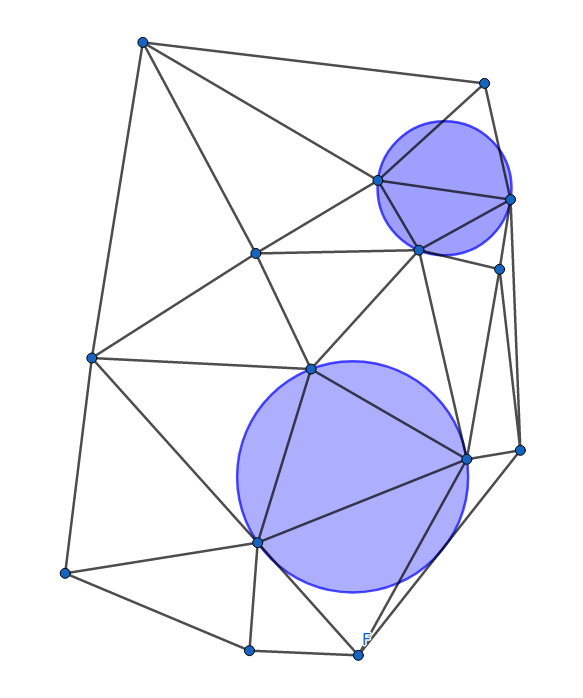
\includegraphics[height = 3cm]{./FigureLayout/DelaunayGood.png}
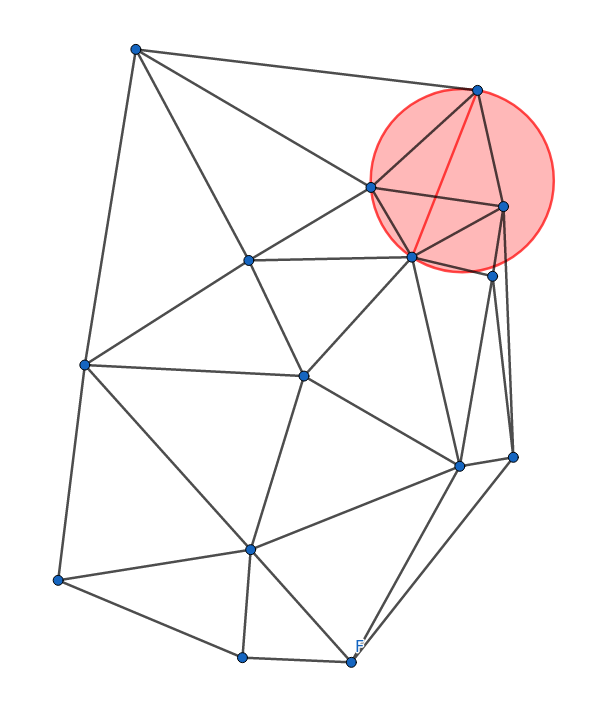
\includegraphics[height = 3cm]{./FigureLayout/DelaunayBad.png}
\end{center}
\end{column}
\begin{column}{0.6\textwidth}
\vspace{10mm}

Additional assumption on $\gamma$ (\alert{No cospherical points}): no $d+2$ points $x_1, \dots, x_{d+2}$ are cospherical, i.e. there is no point $x\in \mathbb R^d$ such that $d(x,x_1)=\dots =d(x,x_d+2)$.\newline

$d(x,y)$ is the Euclidean distance between points $x$ and $y$.
\end{column}
\end{columns}
\end{minipage}
\vspace{3mm}

\mffboxTitle{\textbf{Definition}. Delaunay triangulation in $\mathbb R^d$}{A \alert{Delaunay triangulation} of $\gamma\in\mathcal F_{lf}$ is the set $Del(\gamma)$ defined by
    $$Del(\gamma) = \{T \subset\gamma: \text{card}(T) = d+1,  T \text{ satisfies the empty sphere property } \}.$$
}
\end{small}
\end{frame}


\begin{frame}\frametitle{Delaunay triangulation}\framesubtitle{Through Voronoi tessellation}

For $x \in \gamma$, the \alert{Voronoi cell} of $x$ in $\gamma$ is
$$C(x,\gamma) = \{z \in \mathbb R^d:\; \|x-z\| \leq \|y-z\| \; \forall y \in \gamma \}.$$
\begin{centering}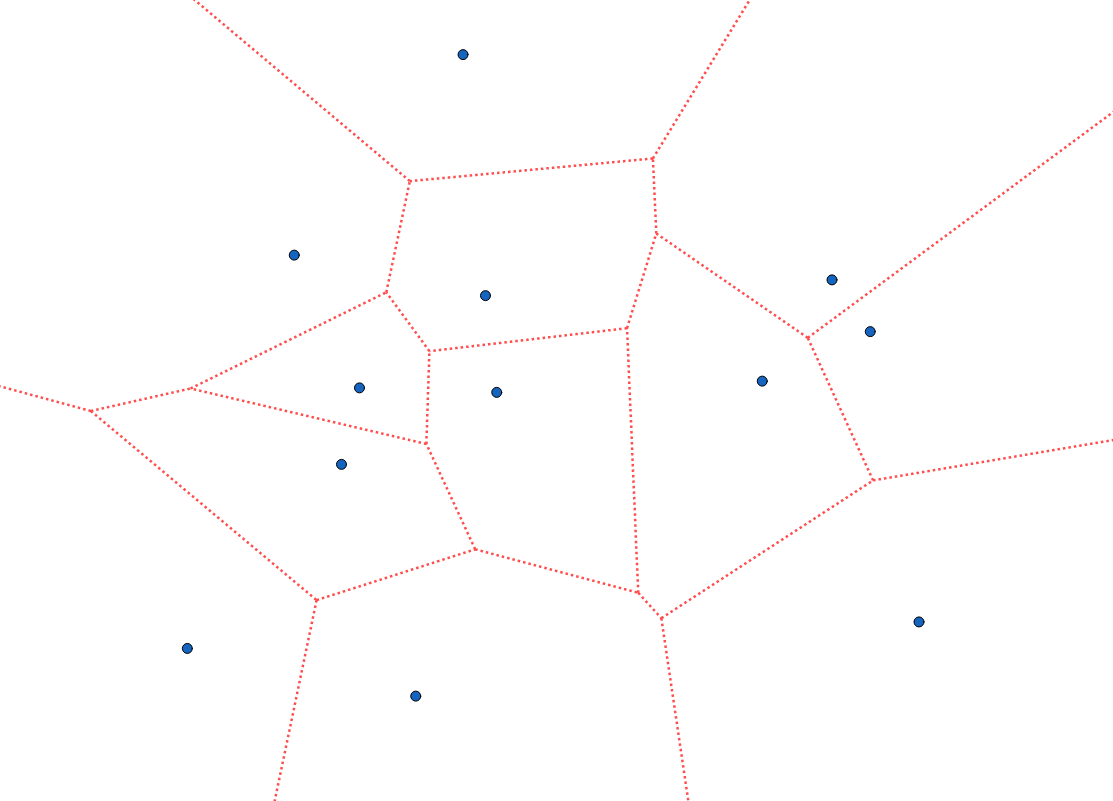
\includegraphics[height = 3.8cm]{./FigureLayout/Voronoi.png}
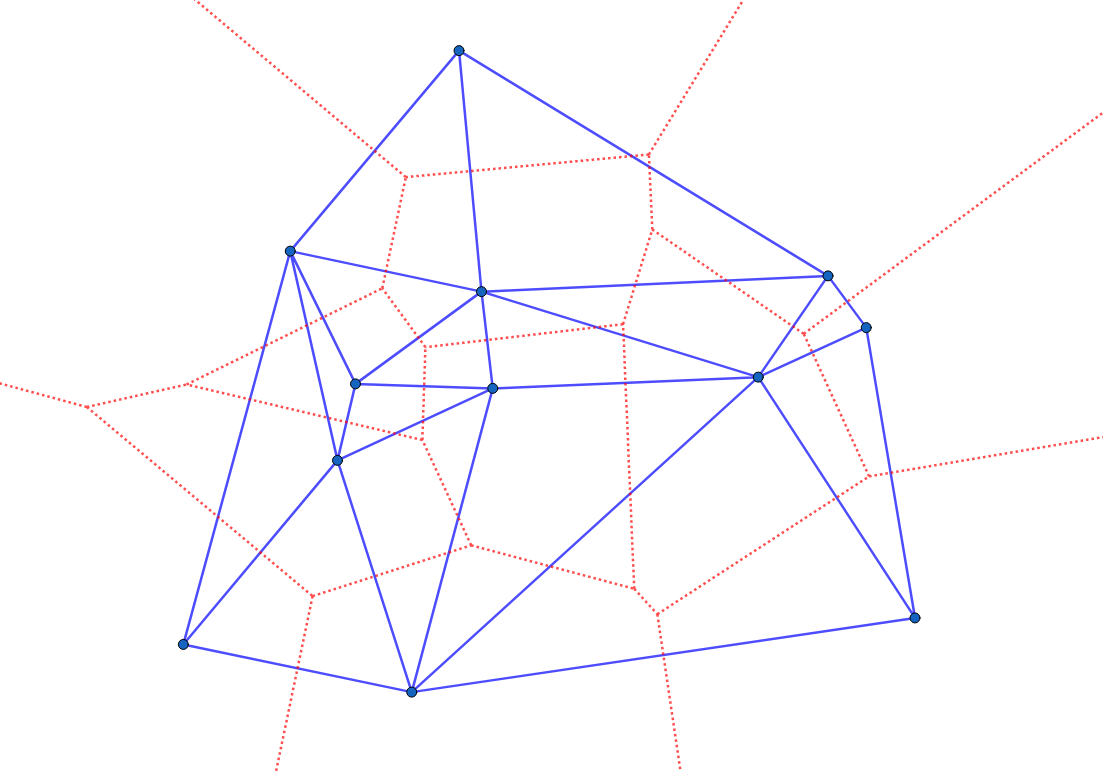
\includegraphics[height = 3.8cm]{./FigureLayout/VoronoiDel.png}\end{centering}
\vspace{3mm}

Then the Delaunay triangulation can be defined as 
$$Del(\gamma) = \{ \{x,y\} \subset \gamma: \; C(x,\gamma)\cap C(y,\gamma) \neq \emptyset \}.$$
\end{frame}





\begin{frame}\frametitle{Delaunay triangulation}\framesubtitle{Building a Delaunay triangulation}
\begin{center}
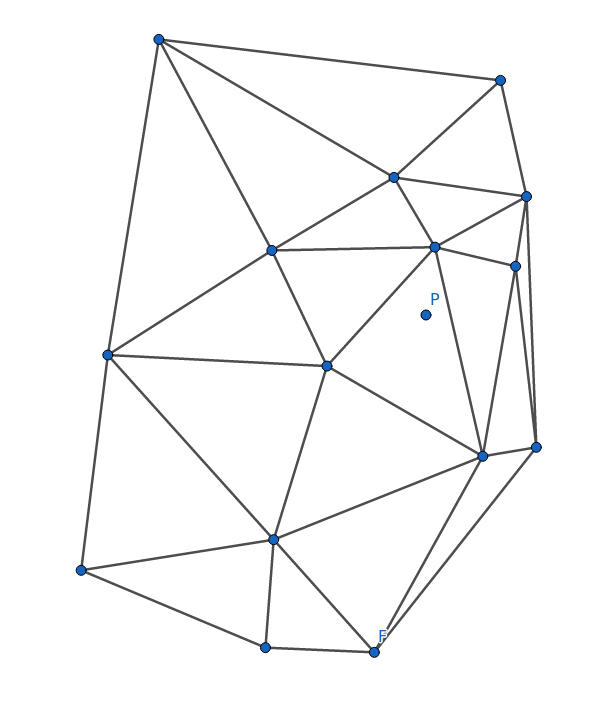
\includegraphics[height = 4cm]{./FigureLayout/DelaunayAdd.png}
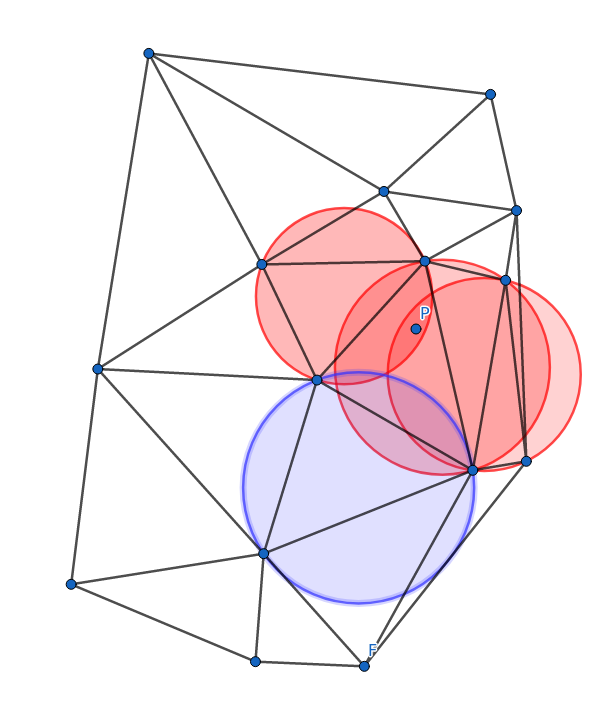
\includegraphics[height = 4cm]{./FigureLayout/DelaunayAdd2.png}
\vspace{1mm}
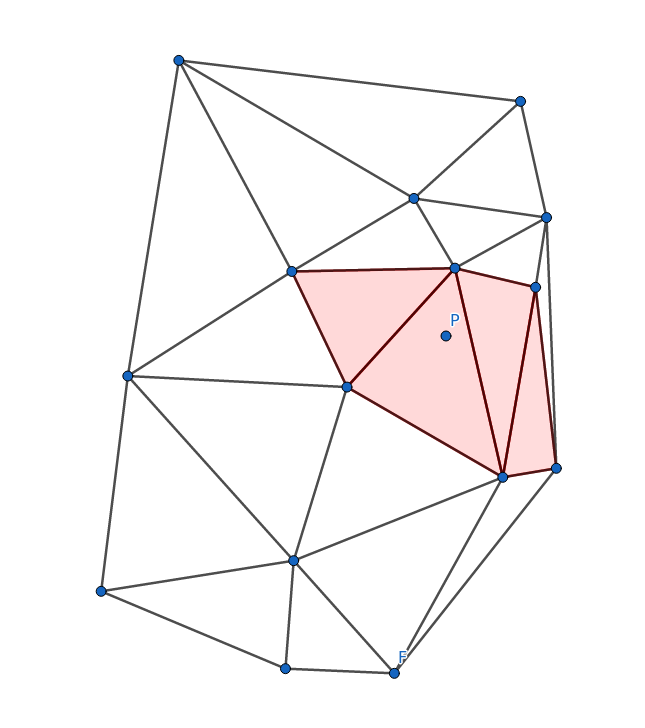
\includegraphics[height = 4.3cm]{./FigureLayout/DelaunayAdd3.png}
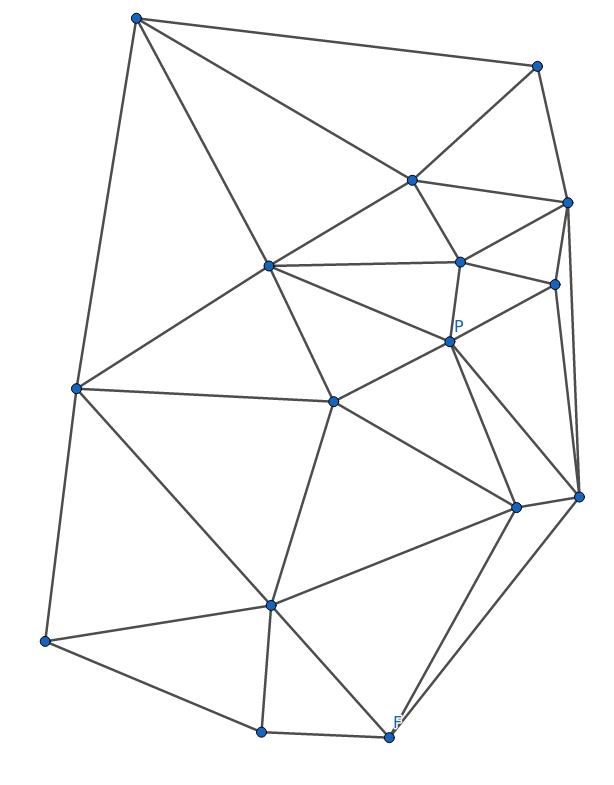
\includegraphics[height = 4cm]{./FigureLayout/DelaunayAdd4.png}
\end{center}


\end{frame}

\begin{frame}\frametitle{Delaunay triangulation in 2D}\framesubtitle{Geometric predicates, 2D}
\begin{small}
In $2D$, with $p_i = (x_i, y_i)$

$$INCIRCLE(p_1,p_2,p_3,p_4) = \begin{vmatrix} x_1 & y_1 & w_1 & 1 \\
x_2 & y_2 & w_2 & 1 \\
x_3 & y_3 &  w_3 & 1 \\
x_4 & y_4 &  w_4 & 1\end{vmatrix}$$

where $w_i = x_i^2  + y_i^2, i = 1,\dots, 4$ and 

$$ORIENTATION(p_1,p_2,p_3) = 
\begin{vmatrix} 
x_1 & y_1 & 1 \\
x_2 & y_2 & 1 \\
x_3 & y_3 & 1 \\
\end{vmatrix} > 0$$
\end{small}

\begin{center}
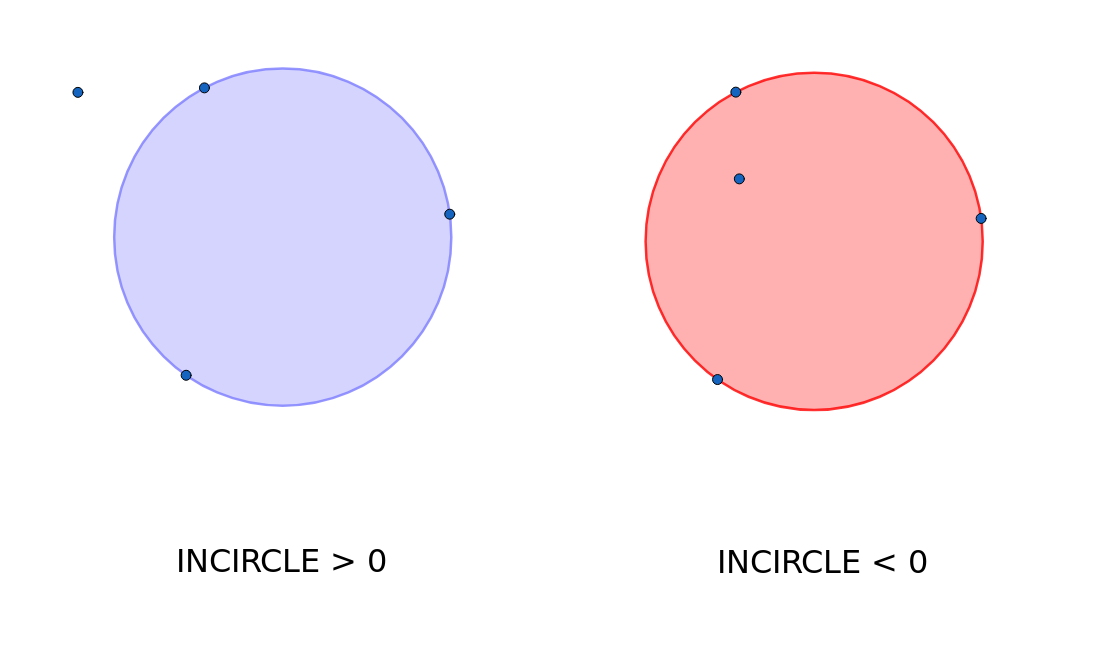
\includegraphics[height = 3cm]{./FigureLayout/Incircle.png}
\end{center}

\end{frame}


\begin{frame}\frametitle{Delaunay triangulation in 3D}\framesubtitle{Geometric predicates, 3D}

In $3D$, with $p_i = ( x_i, y_i, z_i)$

$$INCIRCLE(p_1,p_2,p_3,p_4, p_5) = \begin{vmatrix} x_1 & y_1 & z_1 & w_1 & 1 \\
x_2 & y_2 & z_2 & w_2 & 1 \\
x_3 & y_3 & z_3 & w_3 & 1 \\
x_4 & y_4 & z_4 & w_4 & 1 \\
x_5 & y_5 & z_5 & w_5 & 1\end{vmatrix}$$

where $w_i = x_i^2  + y_i^2 + z_i^2, i = 1,\dots, 5$

if the following condition is satisfied

$$ORIENTATION(p_1,p_2,p_3,p_4) = 
\begin{vmatrix} 
x_1 & y_1 & z_1 & 1 \\
x_2 & y_2 & z_2 & 1 \\
x_3 & y_3 & z_3 & 1 \\
x_4 & y_4 & z_4 & 1 \\
\end{vmatrix} > 0$$

\end{frame}
%%%%% Slide
% ----------------------------------------------------------------------------------------
\begin{frame}\frametitle{Laguerre-Delaunay triangulation}\framesubtitle{Power metric}
\begin{itemize}
\item Generators are not points, but \alert{spheres}. 
\item $\gamma = \{P_1,\dots, P_n\} = \{(p_1, r_{p_1}), \dots , (p_n, r_{p_n})\}$ can be thought of as \alert{marked point process}.
\item Metric is not Euclidean, but \alert{power distance}.
$$ d_p(x,P) = d(x,p)^2 - r_P^2$$
\end{itemize}

\begin{center}
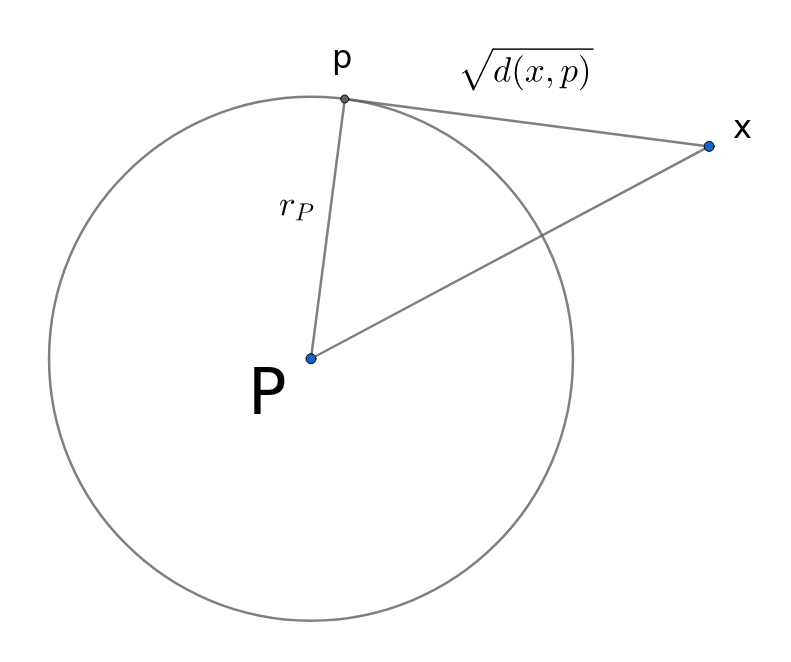
\includegraphics[height = 3.7cm]{./FigureLayout/powerdistance.png}
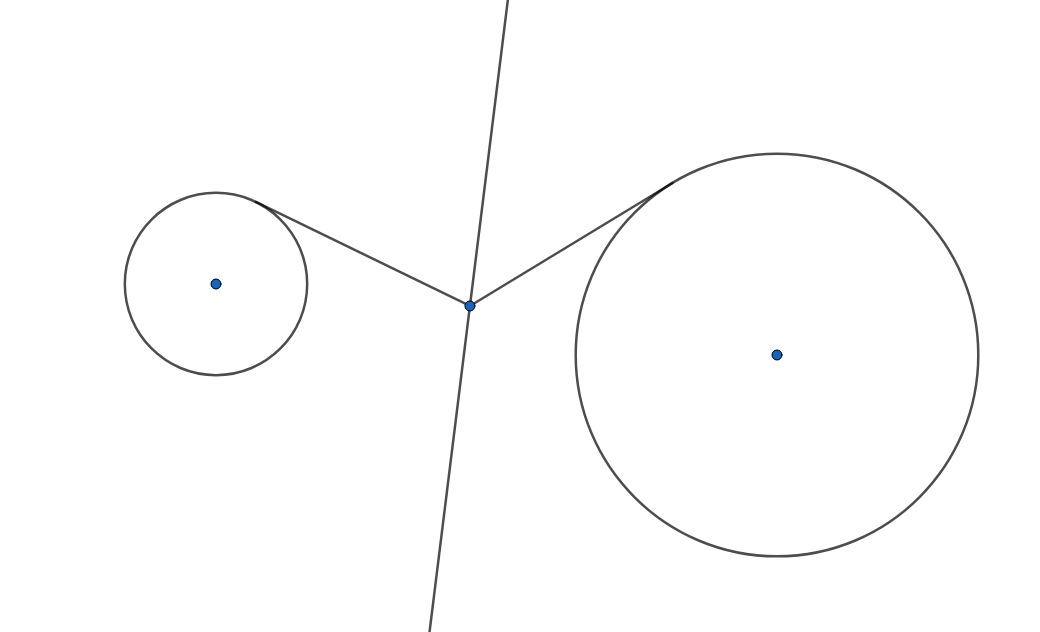
\includegraphics[height = 3.7cm]{./FigureLayout/perpendicularbisector.png}
\end{center}

\end{frame}



\begin{frame}\frametitle{Laguerre-Delaunay triangulation}\framesubtitle{Inscribed sphere and empty sphere property}
\mffboxTitle{\textbf{Definition}. Inscribed sphere}{A sphere $C=(x, \rho)$ is \alert{inscribed} among $d+1$ spheres $P_1, \dots, P_{d+1}$ if
$$ \rho^2 = d_p(x,P_1) = d_p(x,P_2) = \dots = d_p(x, P_{d+1})$$
The spheres $P_1,\dots, P_{d+1}$ are \alert{cospherical} to the sphere $C$.
}

\mffboxTitle{\textbf{Definition}. Empty sphere, empty sphere property}{ The inscribed sphere is called an \alert{empty sphere} if no sphere from $\gamma$ intersects $C$ at an acute angle and if no sphere from $\gamma$ is contained in $C$. 

Spheres $P_{1}, \dots ,P_{d+1}$ satisfy the \alert{empty sphere property} if their inscribed sphere is an empty sphere.
}

\end{frame}


\begin{frame}\frametitle{Laguerre-Delaunay triangulation}\framesubtitle{Definition}
\begin{minipage}[0.2\textheight]{\textwidth}
\begin{columns}[T]
\begin{column}{0.4\textwidth}
\begin{center}
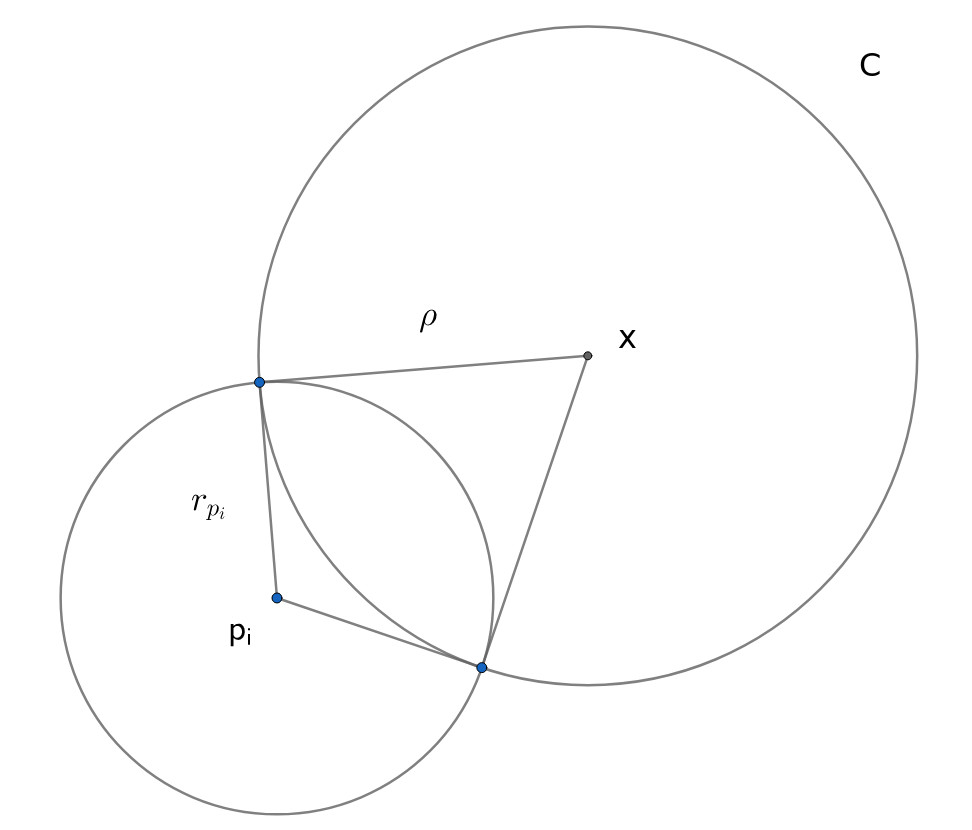
\includegraphics[height = 3.3cm]{./FigureLayout/inscribedsphere.png}
\end{center}
\end{column}
\begin{column}{0.6\textwidth}
\vspace{2cm}

$P_1, \dots, P_{d+1}$ are cospherical $\Rightarrow$ $C$ intersects $P_i, i=1,\dots,d+1$ at a right angle.
\end{column}
\end{columns}
\end{minipage}


\mffboxTitle{\textbf{Definition}. Laguerre-Delaunay triangulation in $\mathbb R^d$}{A \alert{Laguerre-Delaunay triangulation} of a locally finite set $\gamma = \{(p_1, r_{p_1}), \dots , (p_n, r_{p_n})\}$ is the set $\mathcal{L}Del(\gamma)$ defined by
\begin{align*}
    \mathcal LDel(\gamma) &= \{T \subset \gamma:\\
    &\text{card}(T) = d+1,  T \text{ satisfies the empty sphere property } \}.
\end{align*}


}
\end{frame}




\begin{frame}\frametitle{Laguerre-Delaunay triangulation in 3D}\framesubtitle{Geometric predicates, 3D}
\begin{small}
$P_i = (x_i, y_i, z_i, r_i)$

$$INCIRCLE(P_1,P_2,P_3,P_4, P_5) = \begin{vmatrix} x_1 & y_1 & z_1 & w_1 & 1 \\
x_2 & y_2 & z_2 & w_2 & 1 \\
x_3 & y_3 & z_3 & w_3 & 1 \\
x_4 & y_4 & z_4 & w_4 & 1 \\
x_5 & y_5 & z_5 & w_5 & 1\end{vmatrix}$$

where $w_i = x_i^2  + y_i^2 + z_i^2 - \alert{r_i^2}, i = 1,\dots, 5$

if the following condition is satisfied

$$ORIENTATION(P_1,P_2,P_3,P_4) = 
\begin{vmatrix} 
x_1 & y_1 & z_1 & 1 \\
x_2 & y_2 & z_2 & 1 \\
x_3 & y_3 & z_3 & 1 \\
x_4 & y_4 & z_4 & 1 \\
\end{vmatrix} > 0$$

Why? Because both are \alert{regular triangulations} - convex hulls of lifted sets of points, that is
$$\gamma^l = \{(P_i, w_i): P_i \in \gamma, w_i = x_i^2  + y_i^2 + z_i^2 - r_i^2 \}$$

\end{small}
\end{frame}


%%%%% Slide
% ----------------------------------------------------------------------------------------
\begin{frame}\frametitle{Interlude: CGAL}

\begin{center}
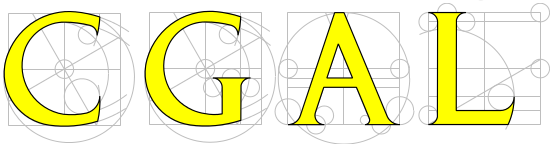
\includegraphics[height = 1cm]{./FigureLayout/cgal.png}
\end{center}

\begin{itemize}
\item Computational Geometry Algorithms Library
\item C++ library for geometric computation.
\item Has fast implementations of both 3D Delaunay and 3D Laguerre-Delaunay triangulations (called Regular triangulation).
\item Offers exact arithmetic for both geometric constructions and geometric predicates.
\end{itemize}


\begin{center}
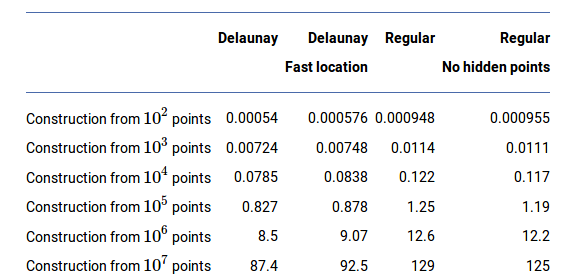
\includegraphics[height = 3cm]{./FigureLayout/cgaltable.png}
\end{center}

\end{frame}




%%%%% Slide
% ----------------------------------------------------------------------------------------
\section{Random triangulations}
\framesection{}


%%%%% Slide
% ----------------------------------------------------------------------------------------
\begin{frame}\frametitle{Poisson-Delaunay triangulation}

\mffboxTitle{\textbf{Definition}. Poisson-Delaunay triangulation in $\mathbb R^d$}{The \alert{Poisson-Delaunay triangulation} of the Poisson point process $\Phi$ is the set $Del(\Phi)$.
}

\begin{center}
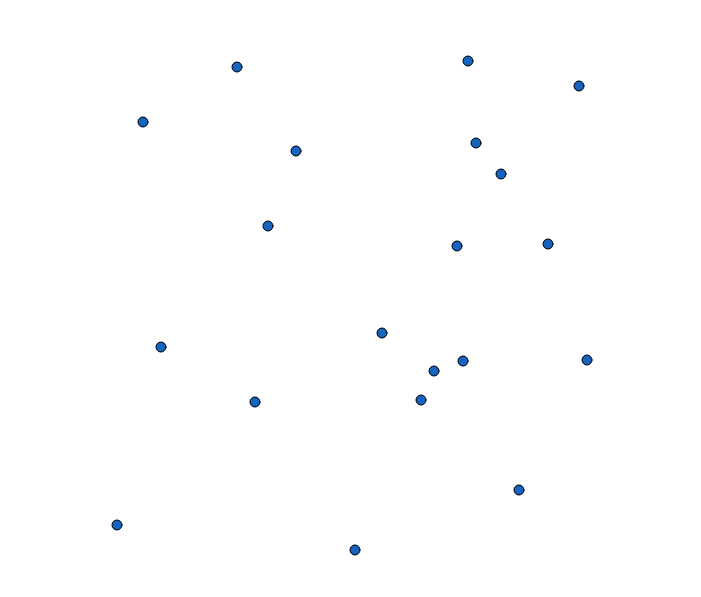
\includegraphics[height = 4.2cm]{./FigureLayout/DelaunayBare.png}
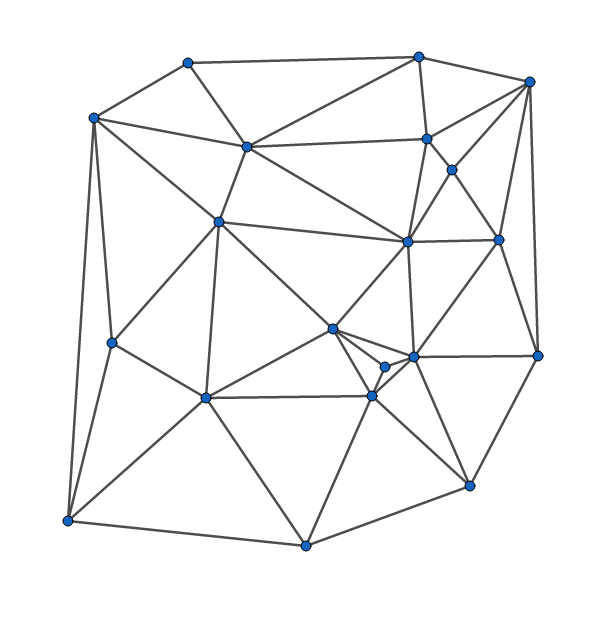
\includegraphics[height = 4.4cm]{./FigureLayout/Delaunay.png}
\end{center}
\end{frame}



%%%%% Slide
% ----------------------------------------------------------------------------------------
\begin{frame}\frametitle{Gibbs-Laguerre-Delaunay triangulation}
\mffboxTitle{\textbf{Definition}. Gibbs-Laguerre-Delaunay triangulation in $\mathbb R^d$}{The \alert{Gibbs-Laguerre-Delaunay triangulation} of the Gibbs point process $\Gamma$ is the set $\mathcal LDel(\Gamma)$
}
\vspace{4mm}

Geometric aspects of the triangulation can be used to define $H$.

In general, the energy can have the form
$$H(\gamma) = \sum_{T \in Del(\gamma)} V_1(T) + \sum_{\{T,T'\} \subset Del (\gamma)} V_2(T,T')$$
to take interaction into account. 
$V_1$ and $V_2$ can be any functions from $d$-dimensional simplices to $\mathbb R \cup \{+ \infty \}$. \newline

\end{frame}




%%%%% Slide
% ----------------------------------------------------------------------------------------
\section{Simulation}
\framesection{}




%%%%% Slide
% ----------------------------------------------------------------------------------------
\begin{frame}\frametitle{Specification of the GLD model}
Our model is the GDL triangulation in $\mathbb R^3$ with  the energy function of the form
$$H(\gamma)= \sum_{T \in Del_\Lambda(\gamma)} V_1(T),$$ 
with $V_1$ defined as
\begin{equation}\label{model}
V_1(T) = 
\left\{
    \begin{array}{ll}
        \infty & \mbox{if } a(T)\leq \epsilon, \\
        \infty & \mbox{if } R(T)\geq \alpha, \\
        \theta Sur(T) & \mbox{otherwise, }
    \end{array}
\right. 
\end{equation}
where
\begin{itemize}
\item $a(T)$ is the area of the smallest face of the tetrahedron $T$.
\item $R(T)$ is the circumradius of $T$.
\item $Sur(T)$ is the surface area of the tetrahedron.
\end{itemize}

Futhermore, $W = [0,W_0]$ is the weight proposal interval, where $W_0>0$ is the maximum weight.

\end{frame}


%%%%% Slide
% ----------------------------------------------------------------------------------------
\begin{frame}\frametitle{Simulating a GLD triangulation}\framesubtitle{Through MCMC}
% Problem: Normalizing constant, need MCMC -> BDM algorithm
% MCMC was invented for Gibbs!
% Initial configuration

\begin{small}
\begin{itemize}
    \item The normalizing constant $C^{z}_\Lambda$ is difficult to obtain.
    \item To sample from the distribution, we use MCMC methods.
    \begin{itemize}
        \item Classic Birth-Death-Move Metropolis-Hastings algorithm, invented for this very purpose.
    \end{itemize} 
\end{itemize}


\textbf{Birth-Death-Move algorithm}\newline
Denote $\Lambda$ the observation window and $\Delta$ the simulation window, $\Lambda \subset \Delta$. $\Lambda_W := \Lambda \times [0,W]$
\begin{enumerate}
    \item Start with a permissible initial configuration $\gamma_0 \subset \Delta \times W$. 
    \item Denote $n=card(\gamma_0\cap \Lambda)$.
    \item In each step, with probability $1/3$:
    \begin{itemize}
        \item \textbf{Birth}: Generate a new point $x \in \Lambda_W$ uniformly. Accept with probability  $ \frac{z f(\gamma_0 \cup \{x\})}{(n+1)f(\gamma_0)},$
        \item \textbf{Death}: Choose $x\in\gamma_0$ uniformly. Accept with probability $ \frac{n f(\gamma_0 \setminus \{x\})}{zf(\gamma_0)},$
        \item \textbf{Move}: Generate a new point $y \in \Lambda_W$ uniformly and choose $x\in\gamma_0$ uniformly. Accept with probability $ \frac{f(\gamma_0 \setminus \{x\} \cup \{y\})}{f(\gamma_0)}.$
    \end{itemize}
    \item Denote the new configuration $\gamma_1$, set $\gamma_0 \leftarrow \gamma_1$ and go to 2.

\end{enumerate}

\end{small}
\end{frame}
 
 
%%%%% Slide
% ----------------------------------------------------------------------------------------
\begin{frame}\frametitle{Comparison with Poisson-Delaunay}
$$ \pi_\Lambda^z \propto z^{N_\Lambda} \pi_\Lambda$$
\vspace{-4mm}
$$ P^{, z}_\Lambda \propto z^{N_\Lambda} \alert{ e^{-\theta H}} \pi_\Lambda $$
\begin{small}$\theta = 0 \Rightarrow$ GPP becomes PPP with intensity $z$.\end{small}
\begin{center}
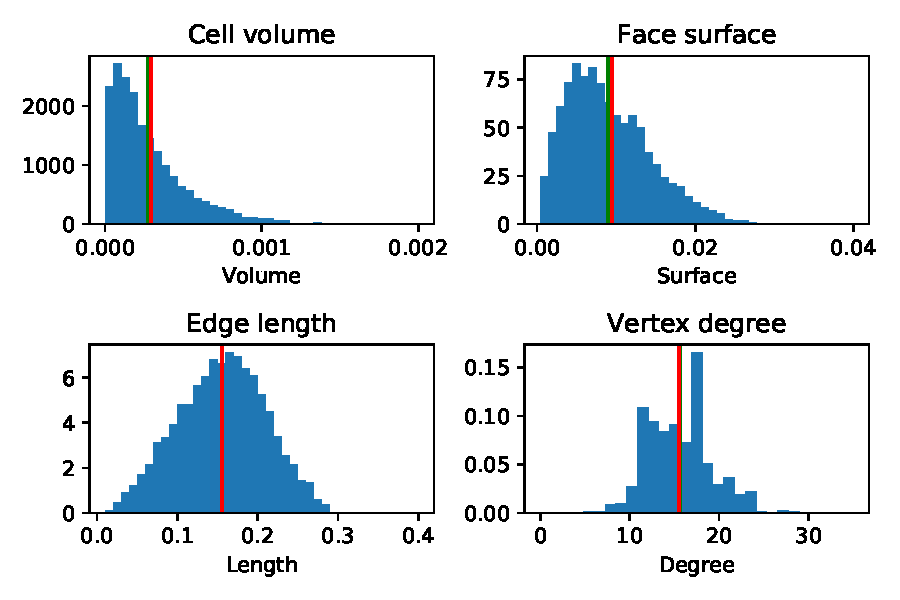
\includegraphics[height = 5.3cm]{./FigureLayout/facets_Poisson.pdf}
\end{center}
\end{frame}




%%%%% Slide
%----------------------------------------------------------------------------------------
\begin{frame}\frametitle{Role of the parameter $\theta$}\framesubtitle{$\theta$ positive}

\begin{small}
The model prefers configurations with lower energy.

$\theta$ multiplies the total surface area of all cells, thus with higher $\theta$, the cells are forced to become large. 
\end{small}
\begin{center}
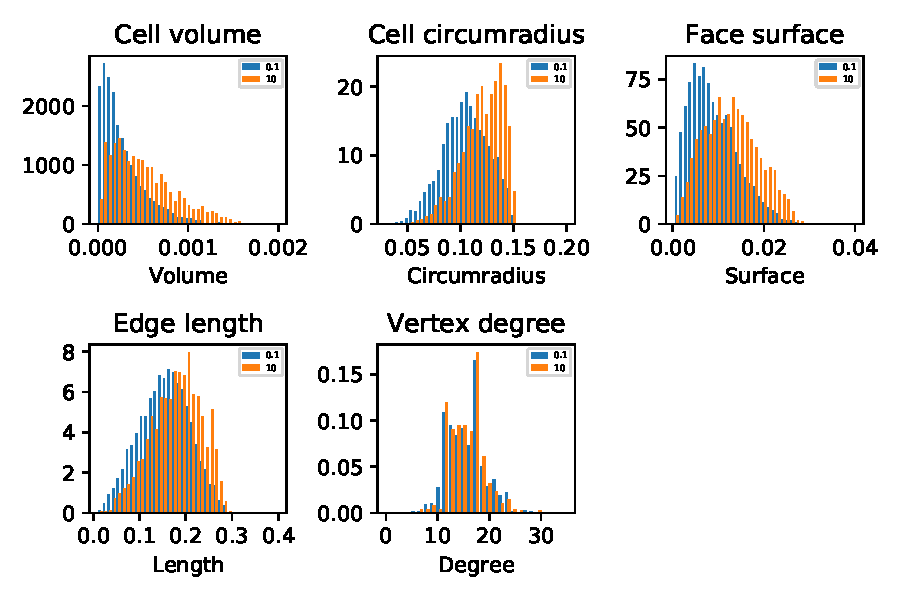
\includegraphics[height = 6.4cm]{./FigureLayout/facets_extr.pdf}
\end{center}

\end{frame}


\begin{frame}\frametitle{Role of the parameter $\theta$}\framesubtitle{$\theta$ negative}
\begin{small}
The model prefers configurations with lower energy.
\begin{itemize}
\item $\theta >0$. The sum needs to be minimized $\Rightarrow$ fewer larger tetrahedra. 
\item $\theta <0$. The sum needs to be maximized $\Rightarrow$ many smaller tetrahedra. 
\end{itemize}
\end{small}

\begin{center}
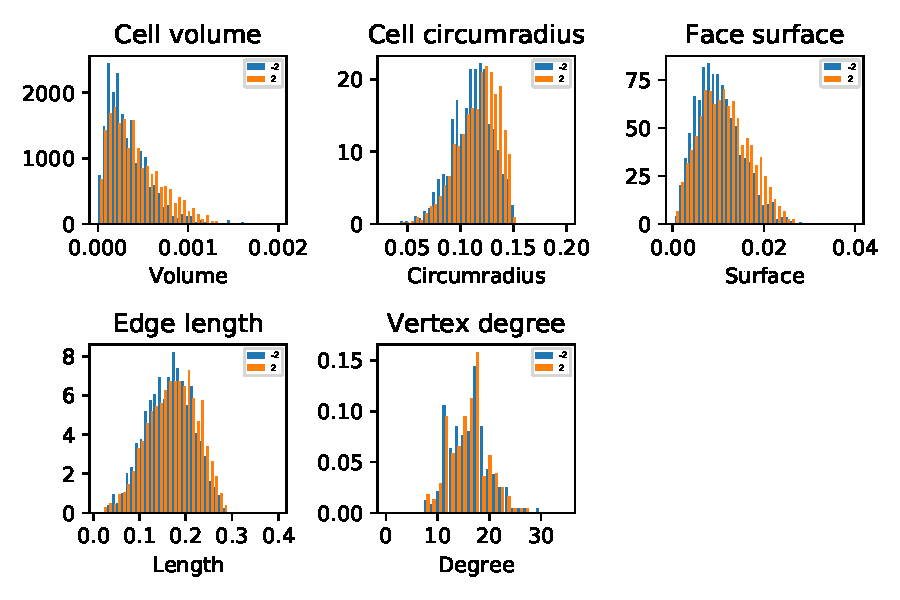
\includegraphics[height = 6cm]{./FigureLayout/facets_neg.pdf}
\end{center}


\end{frame}


%%%%% Slide
% ----------------------------------------------------------------------------------------
\section{Estimation}
\framesection{}




\begin{frame}\frametitle{Two-step procedure}
\begin{small}
We have $4$ parameters to estimate
\begin{itemize}
\item Hard-core parameters.
    \begin{itemize}
    \item The minimum face area $\epsilon$,
    \item the maximum circumradius $\alpha$.
    \end{itemize}
\item Smooth parameters.
    \begin{itemize}
    \item The multiplier of $Sur(T)$, $\theta$,
    \item the intensity of the underlying Poisson point process, $z$.
    \end{itemize}
\end{itemize}
\vspace{5mm}
This is done through a \alert{two-step procedure}
\begin{enumerate}
    \item Estimate the hardcore parameters $(\epsilon, \alpha)$ directly.
    \item Estimate the smooth parameters $(\theta,z)$ by \alert{Maximum Pseudo-Likelihood} (MPLE) using the estimates $(\hat\epsilon,\hat\alpha)$.
\end{enumerate}
\end{small}


\end{frame}

\begin{frame}\frametitle{Two-step procedure}\framesubtitle{1. Hardcore interaction parameters estimation}
\begin{small}
[Dereudre, Lavancier (2009)] only proves consistence for a single parameter (although experimentally both work).\newline

Thanks to the fact that the hardcore parameter $\alpha$ satisfies
$$ \text{if } \alpha < \alpha' \text{ then  } \forall \Lambda, \; H^{\epsilon,\alpha,\theta}_\Lambda(\gamma) < \infty \Rightarrow  H^{\epsilon,\alpha',\theta}_\Lambda(\gamma)<\infty,$$ 
its consistent estimator is
$$\hat\alpha = \sup\{\alpha > 0, H_\Lambda(\gamma) < \infty \},$$
which in practice is estimated as
$$\hat\alpha = \max\{r(T), T\in Del_\Lambda(\gamma)\}.$$

The estimate $\hat\alpha$ is then used in the pseudo-likelihood function in the second estimation step.

\end{small}
\end{frame}


%%%%% Slide
% ----------------------------------------------------------------------------------------
\begin{frame}\frametitle{Two-step procedure}\framesubtitle{2. Maximum pseudolikelihood}
MPLE depends on GNZ, which works only for \alert{hereditary} energy functions.
$$H(\gamma) < \infty \Rightarrow H(\gamma \setminus \{x\}) < \infty \quad x \in \gamma$$

However [Dereudre, Lavancier (2009)] proved that GNZ still holds if we restrict ourselves to \alert{removable points}.\newline

We say a point $x\in \gamma$ is removable if $H(\gamma \setminus \{x\}) < \infty$. Denote $\alert {\mathcal R^\alpha(\gamma)}$ the set of removable points in $\gamma$. 

\begin{center}
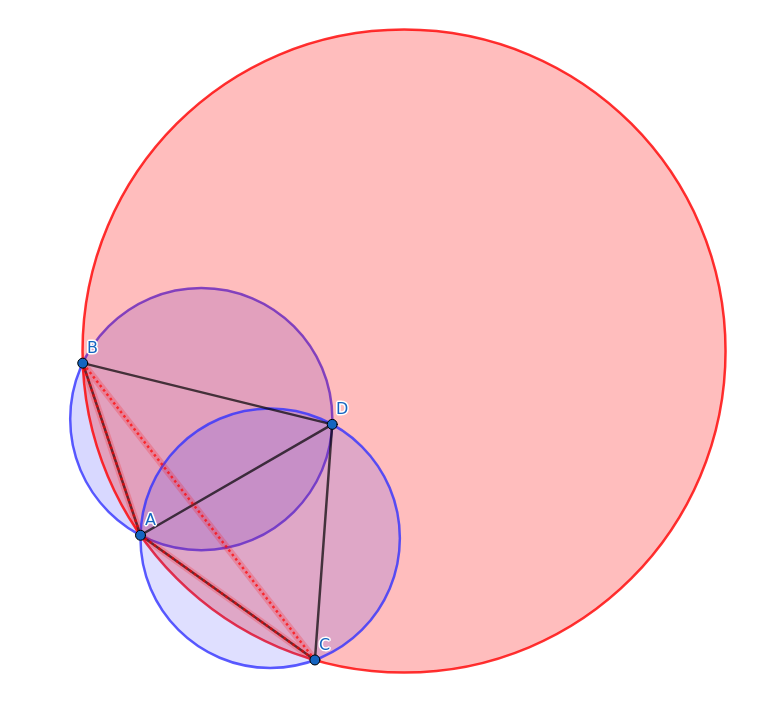
\includegraphics[height = 3.5cm]{./FigureLayout/hereditarity.png}
\end{center}

\end{frame}

%%%%% Slide
% ----------------------------------------------------------------------------------------
\begin{frame}\frametitle{Two-step procedure}\framesubtitle{2. Maximum pseudolikelihood}
\begin{small}
The pseudolikelihood function is
$$ PLL_{\Lambda_W}(\gamma,z,\alpha, \theta) = \int_{\Lambda_W } z \exp (-h^{\alpha,\theta}(x,\gamma)) dx + \sum_{x\in\mathcal R^\alpha(\gamma)\cap \Lambda_W } \big(h^{\alpha,\theta}(x,\gamma\setminus\{x\}) - \ln(z)\big),
$$


The estimates $\hat\theta$ and $\hat z$ are obtained through minimizing the $PLL_{\Lambda_W }$ function. 
$$(\hat z, \hat\theta) = \text{argmin}_{z,\theta} PLL_{\Lambda_W } (\gamma, z, \hat\alpha,\theta).$$

Yielding the estimate $\hat z$ 

$$\hat z = \frac{\mbox{card}(\mathcal R^\alpha(\gamma)\cap \Lambda_W)}{\int_{\Lambda_W} \exp{\left( -h^{\hat\alpha,\theta}(x,\gamma)\right)} dx},$$
and the estimate $\hat\theta$ as the solution of

$$z \int_{\Lambda_W} (h^{\hat\alpha,1}(x,\gamma)\exp{\left(-h^{\hat\alpha,\theta}(x,\gamma)\right)}) dx = \sum_{x \in \mathcal R^{\hat\alpha}(\gamma)\cap \Lambda_W} h^{\hat\alpha,1}(x,\gamma\setminus\{x\}).$$

\end{small}
\end{frame}



\begin{frame}\frametitle{Two-step procedure}\framesubtitle{2. Maximum pseudolikelihood - practical implementation}
\begin{small}
We obtain the estimate of $\theta$ by substituting the expression for $\hat z$ into the equation for $\theta$. 
This leads to the equation
$$ 
\frac{\int_{\Lambda_W } (h^{\hat\alpha,1}(x,\gamma)\exp{\left(-h^{\hat\alpha,\theta}(x,\gamma)\right)}) dx} {  \int_{\Lambda_W } \exp{\left( -h^{\hat\alpha,\theta}(x,\gamma)\right)} dx} 
= \frac {\sum_{x \in \mathcal R^{\hat\alpha}(\gamma)\cap \Lambda_W } h^{\hat\alpha,1}(x,\gamma\setminus\{x\})} { \mbox{card}(\mathcal R^\alpha(\gamma)\cap \Lambda_W ) }. 
$$
After some manipulation, we obtain the equation

$$\int_{\Lambda_W} \exp{\left(-\theta h^{\hat\alpha, 1}(x,\gamma)\right)} (h^{\hat\alpha, 1}(x,\gamma) - c) dx = 0 .$$

After $\hat\theta$ is estimated, we then obtain the estimate $\hat z$ with $\hat\theta$ instead of $\theta$.

All integrals are estimated by MC-integration.
\end{small}
\end{frame}


\begin{frame}\frametitle{Estimation results}\framesubtitle{For Gibbs-Delaunay}
Estimates from $303$ simulations of a Gibbs-Delaunay model with $\theta = 5, z = 500, \alpha = 0.15, \epsilon = 0$

\begin{center}
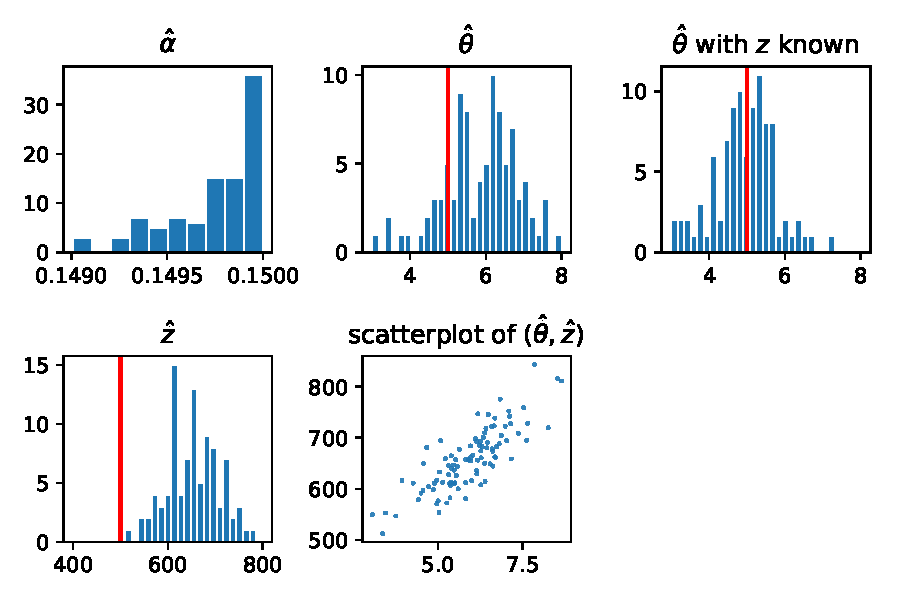
\includegraphics[height = 6cm]{./FigureLayout/estimates_delaunay.pdf}
\end{center}

\end{frame}





\begin{frame}\frametitle{Possible future directions}
\begin{itemize}
\item Variational estimator
$$E \Bigg( \sum_{x \in \Gamma} \nabla_x f(x, \Gamma \setminus \{x\} ) \Bigg) = \theta E \Bigg(\sum_{x \in \Gamma} f(x, \Gamma \setminus \{x\}) \nabla_x h(x, \Gamma \setminus \{x\}) \Bigg).$$
\item Energy with explicit interaction, e.g.
$$V_2(T,T') = \theta \bigg (\frac {\max ( Vol(T), Vol(T'))}{\min(Vol(T),Vol(T'))} - 1\bigg)$$
\item Periodic outside configuration.

\end{itemize}
\end{frame}



% Notes
% No cospherical points assumption



\end{document}
